\chapter{Approach}

\begin{itemize}
	\item Last chapter...
	\item This chapter: Describe shortly all sections from this chapter
	\item In the next chapter...
\end{itemize}

\begin{itemize}
\item In this chapter the practical work should be documented and explained
\item Elaboration of how the practical work could help answer the research question
\item Discussion of real-life setup and how experiments approach it
\end{itemize}





% --------------------------------------------------------
% --------------------------------------------------------
% --------------------------------------------------------
% --------------------------------------------------------



\section{Empirical Research Methods}


\begin{itemize}
\item Overview of methods
\item reproduceability etc.
\item validity
\item Justification why following approaches are conducted as controlled experiments
\end{itemize}

% 2005 Sjoberg: experiments in computer science evaluation

% 2006 Wohlin
% Quantitative: Experiment, Case study, Survey, post-mortem analysis

% 2008_Mytkowicz Observer effect

% 2012 Maxion: Hallmarks of good experiment, Validity

% 2014 Tedre: Experimentation in computing



% --------------------------------------------------------




\subsection{Controlled Experiment}

\begin{itemize}
\item Short overview about controlled experiments in computer science
\item Design: Show test setup image: Independent and dependent variables
\item Hypothesis testing
\end{itemize}

% 2006 Wohlin:
% Design, analysis and interpretation

% 2014 Tedre: Controlled experiments



% --------------------------------------------------------




\subsection{Test Setup}

\begin{itemize}
\item What is test object (website)
\item What are dependent variables: Performance metrics
\item What are independent variables: Specific changes in test object (see next chapter)
\end{itemize}


\paragraph{Measure effects: Dependent Variables}

\begin{itemize}
\item Performance metrics from Lab and Field, see terms and definitions
\item But also quality of RUM data. Because we could have a nice performance but RUM will be of bad quality. 
\end{itemize}


\paragraph{Test object / HTML Template}

\begin{itemize}
\item Depending on different approaches / Ideas (see next chapter), template looks different
\item But general structure stays the same and independent variables can be defined
\item Here we show different independent variables and variants
\end{itemize}


\subsubsection{Lab and Field}

\begin{itemize}
\item I want to collect Lab and field data for dependent variables for comparison
\item This setup is a special case because lab bots (e.g. WPT) simulate at the same time real users for RUM data
\end{itemize}



% --------------------------------------------------------



\subsection{Independent Variables within template}


\begin{itemize}
\item IV 1 POSITION: Position of included analyitcs script. Values: top-head, bottom-head, bottom-body
\item IV 2 ATTRIBUTE: Attribute of included analyitcs script: no-attribute, async, defer
\item IV 3 OTHER SCRIPT: Other tracking script included
\item Other IVs not included but worth mentioning
\end{itemize}




\begin{table}[]
	\centering
	\begin{tabular}{| l | l | }
	\hline
	Variable & Values \\
	\hline
	Position & top-head, bottom-head, bottom-body \\
	Attribute & no attribute, async, defer \\
	Other Script & false, true \\
	\hline
	\end{tabular}
\end{table}

I will compare the values from one independent variable only.
Therefore, when comparing the values of one independent variable, i need to set a default value for the other independent variables.
The default values are:

Position: top-head
Attribute: no attribute
Other Script: false






\paragraph{Other IVs not included but worth mentioning}

\begin{itemize}
\item More or less infinite number of independent variables
\item Again the big and important fact that each website is different
\end{itemize}




% ---- Position ----

% Multiple positions possible

% GA page: 

% From Hotjar installation page: "Paste the Hotjar code into the <head> of every page you wish to track users and collect feedback. And then verify your installation."


\begin{sidewaysfigure}

\begin{multicols}{3}

\begin{center}
\begin{lstlisting}[caption={Position 1}, language=html, numbers=none]
<!DOCTYPE html>
<html>
    <head>
        <!-- Google Analytics -->
        <script></script>
        <!-- End Google Analytics -->

        <title>
        <meta>
        <link>
        <script>
    </head>

    <body>
        ...
    </body>
</html>
\end{lstlisting}
\end{center}

\columnbreak

\begin{center}
\begin{lstlisting}[caption={Position 2}, language=html, numbers=none]
<!DOCTYPE html>
<html>
    <head>
        <title>
        <meta>
        <link>
        <script>
        
        <!-- Google Analytics -->
        <script></script>
        <!-- End Google Analytics -->
    </head>

    <body>
        ...
    </body>
</html>
\end{lstlisting}
\end{center}

\columnbreak

\begin{center}
\begin{lstlisting}[caption={Position 3}, language=html, numbers=none]
<!DOCTYPE html>
<html>
    <head>
        <title>
        <meta>
        <link>
        <script>
        
    </head>

    <body>
        ...
        <!-- Google Analytics -->
        <script></script>
        <!-- End Google Analytics -->
    </body>
</html>
\end{lstlisting}
\end{center}

\end{multicols}

\end{sidewaysfigure}



% ------------------------------------------------------



% Attribute
\begin{sidewaysfigure}

\begin{multicols}{3}

\begin{center}
\begin{lstlisting}[caption={Attribute 1}, language=html, numbers=none]
<!DOCTYPE html>
<html>
    <head>
        <!-- Google Analytics -->
        <script></script>
        <!-- End Google Analytics -->

        <title>
        <meta>
        <link>
        <script>
    </head>

    <body>
        ...
    </body>
</html>
\end{lstlisting}
\end{center}

\columnbreak

\begin{center}
\begin{lstlisting}[caption={Attribute 2}, language=html, numbers=none]
<!DOCTYPE html>
<html>
    <head>
        <!-- Google Analytics -->
        <script async></script>
        <!-- End Google Analytics -->

        <title>
        <meta>
        <link>
        <script>
    </head>

    <body>
        ...
    </body>
</html>
\end{lstlisting}
\end{center}

\columnbreak

\begin{center}
\begin{lstlisting}[caption={Attribute 3}, language=html, numbers=none]
<!DOCTYPE html>
<html>
    <head>
        <!-- Google Analytics -->
        <script defer></script>
        <!-- End Google Analytics -->

        <title>
        <meta>
        <link>
        <script>
    </head>

    <body>
        ...
    </body>
</html>
\end{lstlisting}
\end{center}

\end{multicols}

\end{sidewaysfigure}



% ------------------------------------------------------



% Other Script
\begin{sidewaysfigure}

\begin{multicols}{2}

\begin{center}
\begin{lstlisting}[caption={Other Script 1}, language=html, numbers=none]
<!DOCTYPE html>
<html>
    <head>
        <!-- Google Analytics -->
        <script></script>
        <!-- End Google Analytics -->
        




        <title>
        <meta>
        <link>
        <script>
    </head>

    <body>
        ...
    </body>
</html>
\end{lstlisting}
\end{center}

\columnbreak

\begin{center}
\begin{lstlisting}[caption={Other Script 2}, language=html, numbers=none]
<!DOCTYPE html>
<html>
    <head>
        <!-- Google Analytics -->
        <script></script>
        <!-- End Google Analytics -->
        
        <!-- Other Script-->
        <script></script>
        <!-- End Other Script -->

        <title>
        <meta>
        <link>
        <script>
    </head>

    <body>
        ...
    </body>
</html>
\end{lstlisting}
\end{center}


\end{multicols}

\end{sidewaysfigure}









% --------------------------------------------------------
% --------------------------------------------------------
% --------------------------------------------------------
% --------------------------------------------------------




\section{Test Object: HTML Template / Test website ideas}


\begin{itemize}
\item Several ideas are proposed
\item Each idea has pro and contra: each idea should be discussed of its usefulness, advantages and disadvantages
\end{itemize}



% --------------------------------------------------------


\subsection{WordPress}

\begin{itemize}
    \item Show usage of WordPress with some statistics: Why is it so verbreitet
    \item Explain Plugin system
    \item Explain Setup on localhost with wocommerce and GA plugin
    \item Elaborate why this idea was not used
\end{itemize}




% --------------------------------------------------------



\subsection{Plain / Skeletal Website}

\begin{itemize}
    \item Idea: Lab environment to have control over all and see effects of changing independent variables
    \item Problem: Too far away from reality
    \item Use this as the simplest test possible, not even POC (POC is http archive site)
\end{itemize}




% --------------------------------------------------------



\subsection{HTTP Archive inspired website}

\begin{itemize}
    \item Idea: Get correct page weight
    \item POC: Show that changing independent variables X affect result
\end{itemize}






% --------------------------------------------------------



\subsection{Mirroring a complete e-commerce website}

\paragraph{Otto}

Re-write this to otto start page clone chapter

Manual adjustments:
- Move everything to test folder because top domain is /otto

What did not work (mostly 404s):
- user-set-consent-id-cookie: Cookie with name consentId is not set, user-set-consent-id-cookie returns therefore 404
- subscribeToNewsletterSnippetContent: Change path did not work...
- amount.json: Not found, also wl\_miniWishlistAmount in local storage does not created
- a\_info: Mock a\_info response json does not work...

- footer
- userTiming


WPT RV is returning empty csv when 404s are encountered.
Therefore i mock the missing ressources so that WPT can run bulk tests successfully.

- mock image sprite\_all\_1ba408b2.png

- create empty file called user-set-consent-id-cookie

- change path for subscribeToNewsletterSnippetContent: This will remove the cookie banner... but then WPT works



\begin{itemize}
    \item Idea: Close to reality as possible
    \item Problems when mirroring a website
    \item Elaborate why this idea of mirroring complete website was not used
    \item I used mock of start page of otto, which works fine
    \item Compare original otto website with mock
\end{itemize}





\paragraph{Comparison to original webpage}

\begin{itemize}
    \item Remove GA again from mock, so that mock and original are as similar as possible
    \item Run the same lab test on both pages: WPT and mabye lighthouse
    \item Compare both results and explain differences
\end{itemize}



- Setup: Run WPT on mock and on original website
- WPT config:
- Browser: Chrome
- Number of test runs: 3
- FV and RV
- Capture Video
- Capture DevTools Timeline
- Bulk testing: 100x



Diagrams with FV and RV for both cases:

Technical:
- First Byte
- Bytes In (Doc)
- Requests (Doc)

VIsual:
- Document Complete
- Speed Index

\paragraph{Problem with Repeat View}

- Problem with RV, Caching:
Otto sets request headers to cache-control: no-cache which means that RV basically downloads all resources again.
The mock is hosted on Github, where the cache-control header is set to ...
It is not possible to change the github request headers. We can modify the http request headers via html, but this is not a clean solution.
Therefore I use a different e-commerce website which does not shut down caching so that the RV results are more similar.

Ideally I would host the mock website on a similar infrastructure as the original site with the same webserver configuration. This is for a masters thesis not feasible.

% Not possible to set cache control in html meta tag https://html.spec.whatwg.org/multipage/semantics.html#attr-meta-http-equiv


% --------------------------------------------------------


\paragraph{Zalando}

Idea: It looks like zalando page does not has that many cache-control headers, therefore it may be easier to clone so that RVs are more similar.

Comparison Diagrams with fixed traffic shaping:




% --------------------------------------------------------




\section{Test Runs}

\begin{itemize}
    \item This section covers all conducted test runs
    \item Explain test configuration: how many runs, dependent and independent variables, etc.
\end{itemize}



% --------------------------------------------------------



\subsection{WPT Configurations}


\subsubsection{General Settings}

\begin{table}[h]
	\caption[Test Runs]{Test Runs \cite{DBLP:books/infix/Schwarz99}}
	\label{tab:tamodelleVergleich}
	\centering
	\begin{tabular}{ c | c | c } 
	Configuration Setting & Options & GA \\
	\hline \hline
	Test Location & Test Location & . \\ 
	Browser & Firefox, Chrome & . \\
	\hline
	Connection & LAN & . \\
	Number of Tests to Run & 1 to 9 & .. \\
	Repeat View & First View and Repeat View, First View Only & . \\
	Capture Video & True or False & .. \\
	Keep Test Private & True or False & ... \\
	Label & Any String & ... \\
	\hline	  
	Advanced Tab & ... & ... \\
	Chromium Tab & ... & ... \\
	Auth, Script, Block, SPOF, Custom Tabs & ... & ... \\
	Bulk Testing Tab & List of URLs & ... \\
	\end{tabular}
\end{table}

\paragraph{Explanations}

First View: "First View refers to the cold cache setup in which nothing is served locally"
Repeat View: "Repeat View refers to the warm cache containing everything instantiated by the first view"
(2016 Using WPT p. 62)

Capture Video: ...

\begin{figure}[h!]
  \caption{Number of tests to run: 3, First View and Repeat View}
  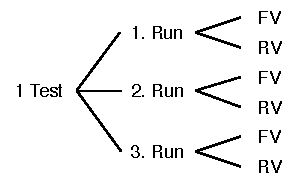
\includegraphics[]{runs}
\end{figure}

For one test, we have actually six times that the website gets loaded and tested.
For e.g. 500 URLs in the bulk test list, we have a total of $500 \times 6 = 3000$ page hits.


\paragraph{Configuration 1}

\begin{table}[h]
	\caption[Test Runs]{Configuration 1}
	\label{tab:tamodelleVergleich}
	\centering
	\begin{tabular}{ |c|c| } 
	\hline
	Configuration Setting & Option \\
	\hline
	Test Location & Test Location \\ 
	Browser & Chrome \\
	\hline
	Connection & LAN \\
	Number of Tests to Run & 3 \\
	Repeat View & First View and Repeat View \\
	Capture Video & True \\
	Keep Test Private & False \\
	Label & none \\
	\hline	  
	Advanced Tab & Nothing selected \\
	Chromium Tab & Nothing selected  \\
	Auth, Script, Block, SPOF, Custom Tabs & Nothing  \\
	Bulk Testing Tab & URL aramyesildeniz... 100 times \\
	\hline
	\end{tabular}
\end{table}

\paragraph{Configuration 2}

Emulate Mobile Browser



\subsubsection{Traffic Shaping}

\begin{itemize}
\item Important to have stable and realistic network condition
\item Chromes tool is not the best for this % see blogpost https://calendar.perfplanet.com/2016/testing-with-realistic-networking-conditions/
\item Private WPT Instance docker on mac does not allow traffic shaping functionality from WPT
\item I use Network Link Conditioner from Apple to slow down the whole machine. See in same blogpost that Patrick highly recommends this
\item WPT also slows down their whole machines % https://forums.webpagetest.org/t/measure-internet-speed/11593
\item IN general internet connection is very unstable. If i run network link conditionier with e.g. DSL each speedtest gives different results. And other test platforms such as fast.com gives also different result.
\end{itemize}





% --------------------------------------------------------



\subsection{Test Object (Website) Variations}

as described before, i will compare the values within one independent variable. 
This is needed in order to compare the impact of the different values within one IV.
For example, i want to measure if there is a difference in performance between the different script attributes. To measure this, i set the default values for the other IVs and vary the values for the IV attribute

Positions:
1: Top of head element
2: just before closing head element
3: just before closing body element


\paragraph{Variants}

\begin{center}
	\begin{longtable}{ |c|c|c|c|  }
	\hline
	Variant & Position & Attribute & Other Scripts \\
	\hline
	Variant P1 & top-head & \cellcolor{lightgrey} none & \cellcolor{lightgrey} no \\
	   Variant P2 & bottom-head & \cellcolor{lightgrey} none & \cellcolor{lightgrey} no \\
	   Variant P3 & bottom-body & \cellcolor{lightgrey} none & \cellcolor{lightgrey} no \\
	  \hline
	   Variant A1 & \cellcolor{lightgrey} top-head & none & \cellcolor{lightgrey} no \\
	   Variant A2 & \cellcolor{lightgrey} top-head & async & \cellcolor{lightgrey} no \\
	   Variant A3 & \cellcolor{lightgrey} top-head & defer & \cellcolor{lightgrey} no \\
	  \hline
	  Variant OS1 & \cellcolor{lightgrey} top-head & \cellcolor{lightgrey} none & no \\
	  Variant OS2 & \cellcolor{lightgrey} top-head & \cellcolor{lightgrey} none & yes \\
	  \hline
	\caption{Your caption here} % needs to go inside longtable environment
	\label{tab:myfirstlongtable}
	\end{longtable}
\end{center}


I will not compare variants which are not from the same subgroup, e.g. Variant A2 will not be compared to Variant OS2.
Because the first row of the variants table also includes the default values for Attribute and Other Scripts, VP1 is equal to VA1 and VO1.

With the defined IVs and variants, I can create the test objects, that is the index.html files with the corresponding setup.
Because its easier to differentiate i will create for the three equal variants nevertheless own index files.

For each test variant, I will create a concrete test artefact, which is a modified index.html.
This index.html needs to be uploaded to the webserver before starting with the tests.

All variants will have the same name which is index.html. This is the default file which will be delivered by the webserver when accessing root path of webpage.



% --------------------------------------------------------


\subsection{Test Plan. Generate the data}

The Google Analytics code is more or less fixed and there are no configurations.
It would be possible to change config of script, e.g. change sample rate, track other metrics etc.
But it is not possible to change default tracking behaviour (?)

How the script is included into the file should reflected withing Website Variations

I will use only one WPT Configuration for all tests.
Other WPT config can be used in future work, e.g. emulate mobile device.


\begin{table}[h]
	\caption[Test Runs]{Test Runs \cite{DBLP:books/infix/Schwarz99}}
	\label{tab:tamodelleVergleich}
	\centering
	\begin{tabular}{ |c|c|c|c| } 
	 \hline
	  Variant & Traffic Shaping & Runs & Date \\
	  \hline
	  V-P1 & DSL & 500 & 2021-05-07 \\
	  V-P2 & DSL & 500 & 2021-05-07 \\
	  V-P3 & DSL & 500 & 2021-05-07 \\
	  \hline
	  V-A1 & DSL & 500 & 2021-05-07 \\
	  V-A2 & DSL & 500 & 2021-05-07 \\
	  V-A3 & DSL & 500 & 2021-05-07 \\
	  \hline
	  V-OS1 & DSL & 500 & 2021-05-07 \\
	  V-OS1 & DSL & 500 & 2021-05-07 \\
	  \hline
	  \end{tabular}
\end{table}



Pre-step: Compare Mock website with and without GA included
The comparison between mock and original is part of chapter Test Object




\subsection{Test Protocol}

\begin{itemize}
\item Deploy variant of index.html by pushing to GitHub
\item Start Network Link Conditioner with specified config on local machine
\item Test internet speed with speedtest-cli
\item Start local WPT server and agent
\item Configure WPT according to specified setup and add list of urls to bulk test interface
\item Run test
\item When finished, download summary csv file
\item On GA helper site, fetch and download data for the current day
\end{itemize}




% --------------------------------------------------------




\subsection{Tool support for diagrams and data analysis}

\begin{itemize}
\item python
\item Matplotlib
\end{itemize}
